% Created 2014-11-17 Mon 15:09
\documentclass[article,10pt,microtype]{article}
\usepackage[utf8]{inputenc}
\usepackage[T1]{fontenc}
\usepackage{fixltx2e}
\usepackage{graphicx}
\usepackage{longtable}
\usepackage{float}
\usepackage{wrapfig}
\usepackage{rotating}
\usepackage[normalem]{ulem}
\usepackage{amsmath}
\usepackage{textcomp}
\usepackage{marvosym}
\usepackage{wasysym}
\usepackage{amssymb}
\usepackage{hyperref}
\tolerance=1000
\usepackage[T1]{fontenc}
\usepackage[T1]{cmap}
\usepackage[english]{babel} % English language/hyphenation
\usepackage{fourier} % Adobe Utopia
\usepackage{ccicons}
\usepackage{sectsty}
\allsectionsfont{\textsc}
\hypersetup{colorlinks=true,urlcolor=blue,linkcolor=blue,pdfborder={0 0 0}}
\usepackage{paralist}
\let\itemize\compactitem
\let\description\compactdesc
\let\enumerate\compactenum
\author{William Denton}
\date{\today}
\title{Reconstructing the AAPR scatterplot data}
\hypersetup{
  pdfkeywords={},
  pdfsubject={},
  pdfcreator={Emacs 25.0.50.2 (Org mode 8.2.10)}}
\begin{document}

\maketitle
The \href{https://yulink.yorku.ca/group/aap/scatterplots/pifs}{scatterplots in the task reports} are available through the \href{https://yulink.yorku.ca/group/aap}{AAPR portal}, but not the raw data that went into constructing them.  This is how I reconstructed it.

(The PDF version of this file is generated from the \href{http://orgmode.org/}{Org mode} file that contains a mix of comment, data and code.  Everything I do to reconstruct the data points is here. Running the code will reproduce what I did.)

I can't make any guarantees about the accuracy of this reconstruction, but it does look to be almost identical.  Corrections and patches are welcome, but the best result would be for the AAPR Task Force to make the raw data available.

\section*{Academic points}
\label{sec-1}

Begin with the academic scatterplots.  They are all laid out exactly the same, as in Figure \ref{fig:academic}, with the chart borders and axes in the same places (except for the close-up view of LA\&PS, which just makes points easier to see).  They look like this:

\begin{figure}[htb]
\centering
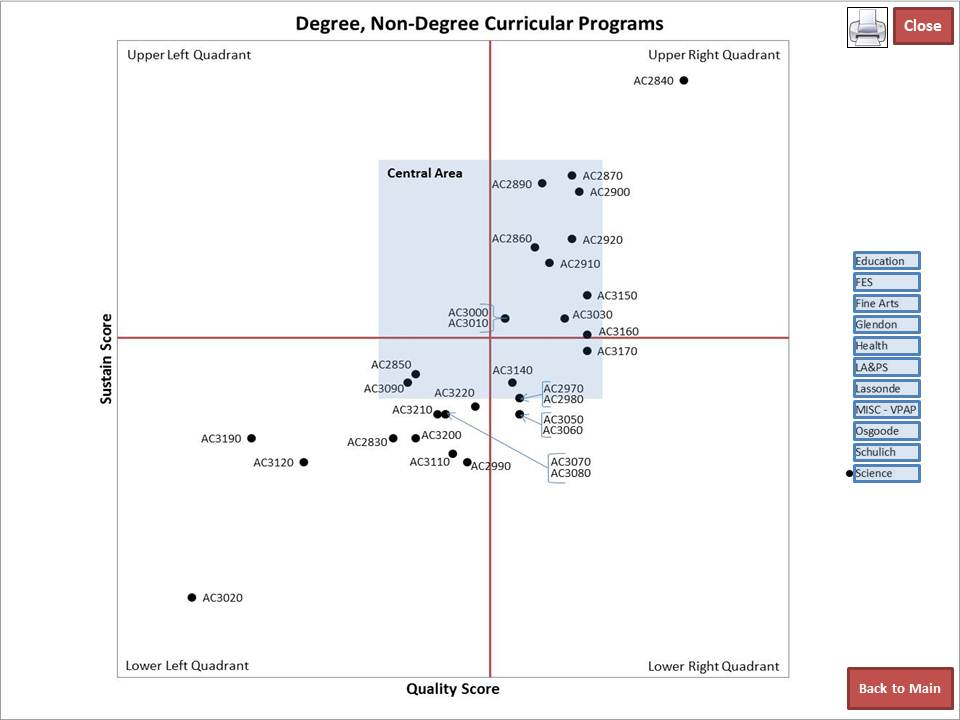
\includegraphics[width=.9\linewidth]{FspAcademicScience.JPG}
\caption{\label{fig:academic}Example academic plot}
\end{figure}

They are all 960 px x 720 px JPEGs.

Let us assume:

\begin{itemize}
\item The scales on both the x- and y-axes go from 1 to 9, inclusive.
\item The charts are linearly scaled on both axes.
\end{itemize}

Using a graphics program we can identify the location of the important pixels in the square bordering the plot (with (0,0) being in the upper right-hand corner of the JPEG; y increases as it goes down):

\begin{center}
\begin{tabular}{lrr}
Point & xpixel & ypixel\\
\hline
Top left & 118 & 40\\
Top right & 788 & 40\\
Bottom left & 118 & 677\\
Bottom right & 788 & 677\\
\end{tabular}
\end{center}

Therefore the width of the x range is \(788 - 118 = 670\) px.  We know this covers the range 1--9, or 8 units of measurement, so each unit is \( 670 / 8 = 83.75\) px wide.  Similarly, the width of the y range is \(677 - 40 = 637\) px, so each unit is \(637 / 8 = 79.625 \) px high.

Thus we can use this formula to convert pixel values to \((Quality, Sustainability)\) values, where \( 1 <= Quality <= 9\) and \(1 <= Sustainability <= 9\).

\begin{equation}
Quality = (xpixel - 118)/83.75 + 1
\end{equation}

\begin{equation}
Sustainability = (677 - ypixel)/79.625 + 1
\end{equation}

We need to add one so that the scales begin at 1, not 0.

This table uses this formula to convert (xpixel, ypixel) to \((Quality, Sustainability)\) for some points of interest, rounded to two decimals:

\begin{longtable}{lrrrr}
\label{testing-calculations}
\\
Point & xpixel & ypixel & Quality & Sustainability\\
\hline
\endhead
\hline\multicolumn{5}{r}{Continued on next page} \\
\endfoot
\endlastfoot
Top left & 118 & 40 & 1 & 9\\
Top right & 788 & 40 & 9 & 9\\
Bottom left & 118 & 677 & 1 & 1\\
Bottom right & 788 & 677 & 9 & 1\\
Central area top left & 378 & 160 & 4.1 & 7.49\\
Central area top right & 600 & 160 & 6.76 & 7.49\\
Central area bottom left & 378 & 398 & 4.1 & 4.5\\
Central area bottom right & 600 & 398 & 6.76 & 4.5\\
Sustainability line left & 118 & 338 & 1 & 5.26\\
Sustainability line right & 788 & 338 & 9 & 5.26\\
Quality line top & 490 & 40 & 5.44 & 9\\
Quality line bottom & 490 & 677 & 5.44 & 1\\
\end{longtable}

Hence we deduce (given our initial assumptions) that the central area covers roughly \(4.1 <= Quality <= 6.75\) and \( 4.5 <= Sustainability <= 7.5\), and that the lines in the middle, perhaps representing acceptable threshold values, are at 5.45 for Quality and 5.25 for Sustainability.

Here are the raw pixel data and the resulting calculated rankings:

\begin{longtable}{llrrrr}
\label{academic}
\\
Image & Code & xpixel & ypixel & Quality & Sustainability\\
\hline
\endhead
\hline\multicolumn{6}{r}{Continued on next page} \\
\endfoot
\endlastfoot
Education & AC0010 & 602 & 217 & 6.78 & 6.78\\
Education & AC0030 & 587 & 328 & 6.6 & 5.38\\
Education & AC0060 & 460 & 375 & 5.08 & 4.79\\
Education & AC0070 & 476 & 397 & 5.27 & 4.52\\
Fes & AC0090 & 510 & 311 & 5.68 & 5.6\\
Fes & AC0110 & 541 & 335 & 6.05 & 5.3\\
Fes & AC0100 & 497 & 382 & 5.53 & 4.7\\
FineArts & AC0310 & 624 & 112 & 7.04 & 8.1\\
FineArts & AC0300 & 602 & 190 & 6.78 & 7.12\\
FineArts & AC0320 & 556 & 255 & 6.23 & 6.3\\
FineArts & AC0190 & 565 & 265 & 6.34 & 6.17\\
FineArts & AC0430 & 587 & 294 & 6.6 & 5.81\\
FineArts & AC0260 & 572 & 303 & 6.42 & 5.7\\
FineArts & AC0250 & 572 & 375 & 6.42 & 4.79\\
FineArts & AC0370 & 541 & 302 & 6.05 & 5.71\\
FineArts & AC0280 & 520 & 285 & 5.8 & 5.92\\
FineArts & AC0350 & 520 & 285 & 5.8 & 5.92\\
FineArts & AC0360 & 520 & 285 & 5.8 & 5.92\\
FineArts & AC0390 & 519 & 304 & 5.79 & 5.68\\
FineArts & AC0400 & 506 & 302 & 5.63 & 5.71\\
FineArts & AC0330 & 529 & 319 & 5.91 & 5.5\\
FineArts & AC0420 & 529 & 340 & 5.91 & 5.23\\
FineArts & AC0270 & 490 & 287 & 5.44 & 5.9\\
FineArts & AC0200 & 490 & 319 & 5.44 & 5.5\\
FineArts & AC0240 & 458 & 238 & 5.06 & 6.51\\
FineArts & AC0220 & 496 & 343 & 5.51 & 5.19\\
FineArts & AC0460 & 504 & 349 & 5.61 & 5.12\\
FineArts & AC0440 & 526 & 351 & 5.87 & 5.09\\
FineArts & AC0140 & 511 & 375 & 5.69 & 4.79\\
FineArts & AC0470 & 547 & 392 & 6.12 & 4.58\\
FineArts & AC0450 & 520 & 392 & 5.8 & 4.58\\
FineArts & AC0170 & 430 & 342 & 4.73 & 5.21\\
FineArts & AC0150 & 475 & 351 & 5.26 & 5.09\\
FineArts & AC0160 & 423 & 389 & 4.64 & 4.62\\
FineArts & AC0130 & 461 & 415 & 5.1 & 4.29\\
Glendon & AC0670 & 527 & 237 & 5.88 & 6.53\\
Glendon & AC0770 & 515 & 255 & 5.74 & 6.3\\
Glendon & AC0790 & 496 & 255 & 5.51 & 6.3\\
Glendon & AC0630 & 531 & 264 & 5.93 & 6.19\\
Glendon & AC0870 & 526 & 278 & 5.87 & 6.01\\
Glendon & AC0610 & 503 & 337 & 5.6 & 5.27\\
Glendon & AC0550 & 475 & 287 & 5.26 & 5.9\\
Glendon & AC0700 & 460 & 285 & 5.08 & 5.92\\
Glendon & AC0750 & 468 & 318 & 5.18 & 5.51\\
Glendon & AC0510 & 445 & 342 & 4.9 & 5.21\\
Glendon & AC0500 & 430 & 345 & 4.73 & 5.17\\
Glendon & AC0860 & 446 & 353 & 4.92 & 5.07\\
Glendon & AC0810 & 424 & 366 & 4.65 & 4.91\\
Glendon & AC0570 & 393 & 375 & 4.28 & 4.79\\
Glendon & AC0680 & 394 & 382 & 4.3 & 4.7\\
Glendon & AC0580 & 355 & 382 & 3.83 & 4.7\\
Glendon & AC0850 & 466 & 390 & 5.16 & 4.6\\
Glendon & AC0530 & 432 & 392 & 4.75 & 4.58\\
Glendon & AC0730 & 432 & 392 & 4.75 & 4.58\\
Glendon & AC0650 & 392 & 430 & 4.27 & 4.1\\
Glendon & AC0830 & 365 & 448 & 3.95 & 3.88\\
Glendon & AC0710 & 452 & 462 & 4.99 & 3.7\\
Glendon & AC0690 & 251 & 533 & 2.59 & 2.81\\
Glendon & AC0590 & 488 & 352 & 5.42 & 5.08\\
Health & AC0920 & 610 & 50 & 6.87 & 8.87\\
Health & AC0980 & 686 & 113 & 7.78 & 8.08\\
Health & AC0990 & 686 & 113 & 7.78 & 8.08\\
Health & AC1060 & 573 & 167 & 6.43 & 7.41\\
Health & AC0930 & 596 & 192 & 6.71 & 7.09\\
Health & AC0940 & 579 & 191 & 6.5 & 7.1\\
Health & AC1130 & 602 & 216 & 6.78 & 6.79\\
Health & AC0960 & 579 & 218 & 6.5 & 6.76\\
Health & AC0950 & 563 & 217 & 6.31 & 6.78\\
Health & AC1120 & 602 & 239 & 6.78 & 6.5\\
Health & AC1000 & 595 & 237 & 6.7 & 6.53\\
Health & AC1030 & 558 & 264 & 6.25 & 6.19\\
Health & AC1010 & 596 & 280 & 6.71 & 5.99\\
Health & AC1020 & 596 & 280 & 6.71 & 5.99\\
Health & AC1070 & 550 & 324 & 6.16 & 5.43\\
Health & AC1050 & 470 & 224 & 5.2 & 6.69\\
Health & AC1100 & 453 & 222 & 5 & 6.71\\
Health & AC1110 & 453 & 222 & 5 & 6.71\\
Health & AC1080 & 420 & 389 & 4.61 & 4.62\\
Lassonde & AC2480 & 572 & 129 & 6.42 & 7.88\\
Lassonde & AC2490 & 572 & 129 & 6.42 & 7.88\\
Lassonde & AC2640 & 548 & 241 & 6.13 & 6.48\\
Lassonde & AC2520 & 527 & 278 & 5.88 & 6.01\\
Lassonde & AC2530 & 527 & 278 & 5.88 & 6.01\\
Lassonde & AC2460 & 528 & 325 & 5.9 & 5.42\\
Lassonde & AC2500 & 528 & 325 & 5.9 & 5.42\\
Lassonde & AC2510 & 528 & 325 & 5.9 & 5.42\\
Lassonde & AC2550 & 492 & 326 & 5.47 & 5.41\\
Lassonde & AC2560 & 496 & 342 & 5.51 & 5.21\\
Lassonde & AC2600 & 505 & 368 & 5.62 & 4.88\\
Lassonde & AC2610 & 505 & 368 & 5.62 & 4.88\\
Lassonde & AC2470 & 524 & 398 & 5.85 & 4.5\\
Lassonde & AC2590 & 490 & 415 & 5.44 & 4.29\\
Lassonde & AC2570 & 502 & 462 & 5.59 & 3.7\\
Laps & AC2090 & 490 & 86 & 5.44 & 8.42\\
Laps & AC1390 & 490 & 135 & 5.44 & 7.81\\
Laps & AC2230 & 370 & 270 & 4.01 & 6.11\\
Laps & AC2340 & 622 & 286 & 7.02 & 5.91\\
Laps & AC1510 & 473 & 406 & 5.24 & 4.4\\
Laps & AC2940 & 473 & 406 & 5.24 & 4.4\\
Laps & AC1320 & 475 & 414 & 5.26 & 4.3\\
Laps & AC1560 & 490 & 414 & 5.44 & 4.3\\
Laps & AC1570 & 490 & 414 & 5.44 & 4.3\\
Laps & AC1440 & 608 & 351 & 6.85 & 5.09\\
Laps & AC1680 & 526 & 413 & 5.87 & 4.32\\
Laps & AC1600 & 550 & 414 & 6.16 & 4.3\\
Laps & AC1660 & 526 & 446 & 5.87 & 3.9\\
Laps & AC1260 & 527 & 454 & 5.88 & 3.8\\
Laps & AC2020 & 565 & 444 & 6.34 & 3.93\\
Laps & AC2300 & 467 & 430 & 5.17 & 4.1\\
Laps & AC2310 & 467 & 430 & 5.17 & 4.1\\
Laps & AC2040 & 453 & 429 & 5 & 4.11\\
Laps & AC1830 & 437 & 430 & 4.81 & 4.1\\
Laps & AC2250 & 401 & 414 & 4.38 & 4.3\\
Laps & AC1790 & 416 & 429 & 4.56 & 4.11\\
Laps & AC1849 & 416 & 429 & 4.56 & 4.11\\
Laps & AC2110 & 416 & 438 & 4.56 & 4\\
Laps & AC2950 & 421 & 437 & 4.62 & 4.01\\
Laps & AC2010 & 459 & 439 & 5.07 & 3.99\\
Laps & AC1280 & 474 & 455 & 5.25 & 3.79\\
Laps & AC1610 & 444 & 462 & 4.89 & 3.7\\
Laps & AC1490 & 452 & 462 & 4.99 & 3.7\\
Laps & AC1270 & 476 & 510 & 5.27 & 3.1\\
Laps & AC1760 & 365 & 409 & 3.95 & 4.37\\
Laps & AC2130 & 355 & 422 & 3.83 & 4.2\\
Laps & AC2060 & 379 & 446 & 4.12 & 3.9\\
Laps & AC1550 & 393 & 450 & 4.28 & 3.85\\
Laps & AC1850 & 416 & 478 & 4.56 & 3.5\\
Laps & AC1310 & 430 & 487 & 4.73 & 3.39\\
Laps & AC1350 & 398 & 486 & 4.34 & 3.4\\
Laps & AC1770 & 407 & 510 & 4.45 & 3.1\\
Laps & AC2150 & 346 & 486 & 3.72 & 3.4\\
Laps & AC2100 & 335 & 497 & 3.59 & 3.26\\
Laps & AC1740 & 303 & 502 & 3.21 & 3.2\\
Laps & AC1800 & 295 & 542 & 3.11 & 2.7\\
Laps & AC1820 & 304 & 542 & 3.22 & 2.7\\
Laps & AC2200 & 325 & 552 & 3.47 & 2.57\\
Laps & AC2240 & 354 & 550 & 3.82 & 2.59\\
Laps & AC2160 & 444 & 184 & 4.89 & 7.19\\
Laps & AC1480 & 468 & 206 & 5.18 & 6.92\\
Laps & AC1700 & 550 & 181 & 6.16 & 7.23\\
Laps & AC1230 & 557 & 193 & 6.24 & 7.08\\
Laps & AC1240 & 557 & 193 & 6.24 & 7.08\\
Laps & AC1710 & 490 & 207 & 5.44 & 6.9\\
Laps & AC2170 & 505 & 216 & 5.62 & 6.79\\
Laps & AC2420 & 505 & 224 & 5.62 & 6.69\\
Laps & AC2430 & 505 & 224 & 5.62 & 6.69\\
Laps & AC1380 & 482 & 232 & 5.35 & 6.59\\
Laps & AC1400 & 490 & 232 & 5.44 & 6.59\\
Laps & AC1220 & 504 & 238 & 5.61 & 6.51\\
Laps & AC2180 & 490 & 262 & 5.44 & 6.21\\
Laps & AC1300 & 526 & 261 & 5.87 & 6.22\\
Laps & AC2435 & 452 & 270 & 4.99 & 6.11\\
Laps & AC1810 & 484 & 270 & 5.37 & 6.11\\
Laps & AC2190 & 490 & 278 & 5.44 & 6.01\\
Laps & AC1180 & 565 & 286 & 6.34 & 5.91\\
Laps & AC1960 & 467 & 310 & 5.17 & 5.61\\
Laps & AC2210 & 453 & 318 & 5 & 5.51\\
Laps & AC1420 & 430 & 334 & 4.73 & 5.31\\
Laps & AC2380 & 512 & 310 & 5.7 & 5.61\\
Laps & AC1200 & 512 & 326 & 5.7 & 5.41\\
Laps & AC1890 & 506 & 333 & 5.63 & 5.32\\
Laps & AC1900 & 526 & 334 & 5.87 & 5.31\\
Laps & AC1430 & 378 & 383 & 4.1 & 4.69\\
Laps & AC1355 & 416 & 350 & 4.56 & 5.11\\
Laps & AC2030 & 417 & 367 & 4.57 & 4.89\\
Laps & AC1540 & 431 & 390 & 4.74 & 4.6\\
Laps & AC1950 & 431 & 390 & 4.74 & 4.6\\
Laps & AC2090 & 431 & 390 & 4.74 & 4.6\\
Laps & AC1920 & 452 & 358 & 4.99 & 5.01\\
Laps & AC1325 & 454 & 366 & 5.01 & 4.91\\
Laps & AC1930 & 454 & 366 & 5.01 & 4.91\\
Laps & AC2120 & 454 & 366 & 5.01 & 4.91\\
Laps & AC1290 & 468 & 368 & 5.18 & 4.88\\
Laps & AC1910 & 468 & 368 & 5.18 & 4.88\\
Laps & AC1630 & 476 & 372 & 5.27 & 4.83\\
Laps & AC1540 & 430 & 390 & 4.73 & 4.6\\
Laps & AC1950 & 430 & 390 & 4.73 & 4.6\\
Laps & AC2090 & 430 & 390 & 4.73 & 4.6\\
Laps & AC2280 & 446 & 398 & 4.92 & 4.5\\
Laps & AC1780 & 454 & 398 & 5.01 & 4.5\\
Laps & AC1970 & 466 & 391 & 5.16 & 4.59\\
Laps & AC2360 & 466 & 391 & 5.16 & 4.59\\
Laps & AC2270 & 476 & 390 & 5.27 & 4.6\\
Laps & AC1980 & 484 & 390 & 5.37 & 4.6\\
Laps & AC2260 & 490 & 342 & 5.44 & 5.21\\
Laps & AC1620 & 490 & 352 & 5.44 & 5.08\\
Laps & AC1640 & 490 & 352 & 5.44 & 5.08\\
Laps & AC1360 & 490 & 366 & 5.44 & 4.91\\
Laps & AC2400 & 490 & 366 & 5.44 & 4.91\\
Laps & AC1190 & 498 & 350 & 5.54 & 5.11\\
Laps & AC2290 & 506 & 351 & 5.63 & 5.09\\
Laps & AC2390 & 512 & 350 & 5.7 & 5.11\\
Laps & AC1750 & 549 & 350 & 6.15 & 5.11\\
Laps & AC1460 & 550 & 358 & 6.16 & 5.01\\
Laps & AC1470 & 565 & 352 & 6.34 & 5.08\\
Laps & AC1720 & 504 & 366 & 5.61 & 4.91\\
Laps & AC1370 & 512 & 365 & 5.7 & 4.92\\
Laps & AC2350 & 512 & 365 & 5.7 & 4.92\\
Laps & AC1450 & 506 & 374 & 5.63 & 4.81\\
Laps & AC1670 & 526 & 390 & 5.87 & 4.6\\
Misc & AC3360 & 406 & 382 & 4.44 & 4.7\\
Osgoode & AC2670 & 662 & 105 & 7.5 & 8.18\\
Osgoode & AC2690 & 572 & 297 & 6.42 & 5.77\\
Osgoode & AC2680 & 536 & 320 & 5.99 & 5.48\\
Schulich & AC2760 & 726 & 136 & 8.26 & 7.79\\
Schulich & AC2740 & 698 & 168 & 7.93 & 7.39\\
Schulich & AC2780 & 586 & 192 & 6.59 & 7.09\\
Schulich & AC2810 & 549 & 340 & 6.15 & 5.23\\
Science & AC2840 & 683 & 81 & 7.75 & 8.49\\
Science & AC2870 & 570 & 178 & 6.4 & 7.27\\
Science & AC2890 & 542 & 183 & 6.06 & 7.2\\
Science & AC2900 & 579 & 192 & 6.5 & 7.09\\
Science & AC2920 & 571 & 236 & 6.41 & 6.54\\
Science & AC2860 & 534 & 245 & 5.97 & 6.43\\
Science & AC2910 & 548 & 263 & 6.13 & 6.2\\
Science & AC3150 & 586 & 294 & 6.59 & 5.81\\
Science & AC3030 & 564 & 320 & 6.33 & 5.48\\
Science & AC3000 & 505 & 318 & 5.62 & 5.51\\
Science & AC3010 & 505 & 318 & 5.62 & 5.51\\
Science & AC3160 & 587 & 333 & 6.6 & 5.32\\
Science & AC3170 & 586 & 349 & 6.59 & 5.12\\
Science & AC3140 & 510 & 382 & 5.68 & 4.7\\
Science & AC2970 & 518 & 399 & 5.78 & 4.49\\
Science & AC2980 & 518 & 399 & 5.78 & 4.49\\
Science & AC3050 & 519 & 415 & 5.79 & 4.29\\
Science & AC3060 & 519 & 415 & 5.79 & 4.29\\
Science & AC2850 & 414 & 372 & 4.53 & 4.83\\
Science & AC3090 & 406 & 383 & 4.44 & 4.69\\
Science & AC3220 & 473 & 407 & 5.24 & 4.39\\
Science & AC3210 & 436 & 415 & 4.8 & 4.29\\
Science & AC3070 & 444 & 414 & 4.89 & 4.3\\
Science & AC3080 & 444 & 414 & 4.89 & 4.3\\
Science & AC3200 & 415 & 439 & 4.55 & 3.99\\
Science & AC3110 & 454 & 452 & 5.01 & 3.83\\
Science & AC2990 & 466 & 462 & 5.16 & 3.7\\
Science & AC2830 & 393 & 439 & 4.28 & 3.99\\
Science & AC3120 & 302 & 464 & 3.2 & 3.68\\
Science & AC3190 & 251 & 440 & 2.59 & 3.98\\
Science & AC3020 & 190 & 597 & 1.86 & 2\\
\end{longtable}

A short Ruby script takes that data and generates \texttt{aapr-academic.csv}:

\begin{verbatim}
File.open("aapr-academic.csv", "w") { |f|
  f.write "Program_Code,Quality,Sustainability\n"
  table.each do |r|
    f.write "#{r[1]},#{r[4]},#{r[5]}\n"
  end
}
\end{verbatim}


\section*{Administrative points}
\label{sec-2}

These images are also 960 px x 720 px, but the bounding box is different (see Fig \ref{fig:administrative}) so we need to do fresh calculations.

\begin{figure}[htb]
\centering
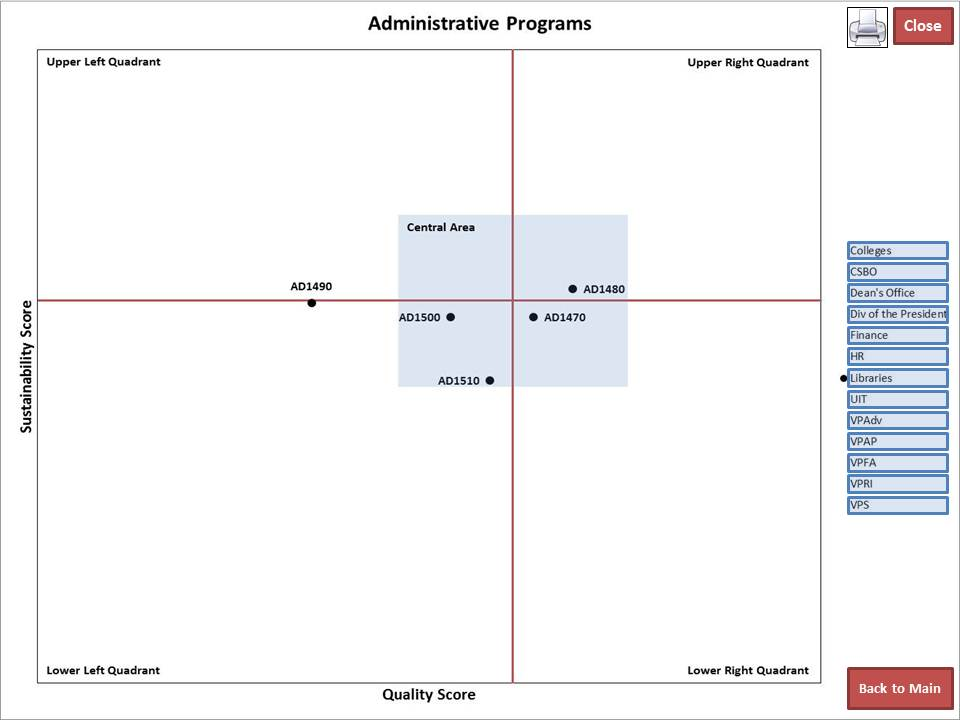
\includegraphics[width=.9\linewidth]{FspAdministrativeLibraries.JPG}
\caption{\label{fig:administrative}Example administrative plot}
\end{figure}

\begin{center}
\begin{tabular}{lrr}
Point & xpixel & ypixel\\
\hline
Top left & 38 & 48\\
Top right & 820 & 48\\
Bottom left & 38 & 682\\
Bottom right & 820 & 682\\
\end{tabular}
\end{center}

The width of the x range is \(820 - 38 = 782\) px.  Again we know this covers the range 1--9, or 8 units of measurement, so each unit is \( 782 / 8 = 97.75\) px wide.  Similarly, the width of the y range is \(682 - 48 = 634\) px, and each unit is \(634 / 8 = 79.25 \) px high.

Thus we can use this formula to convert pixel values to \((Quality, Sustainability)\) values, where \( 1 <= Quality <= 9\) and \(1 <= Sustainability <= 9\).

\begin{equation}
Quality = (xpixel - 38)/97.75 + 1
\end{equation}

\begin{equation}
Sustainability = (682 - ypixel)/79.25 + 1
\end{equation}

We need to add one so that the scales begin at 1, not 0.

This table uses this formula to convert (xpixel, ypixel) to \((Quality, Sustainability)\) for some points of interest, rounded to two decimals:

\begin{center}
\begin{tabular}{lrrrr}
Point & xpixel & ypixel & Quality & Sustainability\\
\hline
Top left & 38 & 48 & 1 & 9\\
Top right & 820 & 48 & 9 & 9\\
Bottom left & 38 & 682 & 1 & 1\\
Bottom right & 820 & 682 & 9 & 1\\
Central area top left & 398 & 213 & 4.68 & 6.92\\
Central area top right & 628 & 213 & 7.04 & 6.92\\
Central area bottom left & 398 & 384 & 4.68 & 4.76\\
Central area bottom right & 628 & 384 & 7.04 & 4.76\\
Sustainability line left & 38 & 300 & 1 & 5.82\\
Sustainability line right & 820 & 300 & 9 & 5.82\\
Quality line top & 512 & 48 & 5.85 & 9\\
Quality line bottom & 512 & 682 & 5.85 & 1\\
\end{tabular}
\end{center}

Here the Sustainability threshold is about 5.8 and the Quality threshold is 5.85.

Here are the raw pixel data and the resulting calculated rankings:

\begin{longtable}{llrrrr}
\label{administrative}
\\
Image & Code & xpixel & ypixel & Quality & Sustainability\\
\hline
\endhead
\hline\multicolumn{6}{r}{Continued on next page} \\
\endfoot
\endlastfoot
Colleges & AD1320 & 622 & 323 & 7.02 & 5.45\\
Colleges & AD1330 & 622 & 323 & 7.02 & 5.45\\
Colleges & AD1530 & 581 & 369 & 6.53 & 4.87\\
Colleges & AD1380 & 478 & 390 & 5.3 & 4.6\\
Colleges & AD1260 & 411 & 404 & 4.5 & 4.43\\
Colleges & AD1400 & 433 & 460 & 4.76 & 3.73\\
Colleges & AD1370 & 332 & 495 & 3.56 & 3.29\\
Colleges & AD1390 & 329 & 493 & 3.52 & 3.31\\
Csbo & AD0950 & 560 & 186 & 6.28 & 7.17\\
Csbo & AD1090 & 581 & 190 & 6.53 & 7.12\\
Csbo & AD1100 & 581 & 190 & 6.53 & 7.12\\
Csbo & AD1110 & 589 & 247 & 6.62 & 6.4\\
Csbo & AD1050 & 545 & 255 & 6.1 & 6.3\\
Csbo & AD1160 & 606 & 272 & 6.83 & 6.09\\
Csbo & AD0960 & 517 & 298 & 5.76 & 5.76\\
Csbo & AD1130 & 474 & 238 & 5.25 & 6.51\\
Csbo & AD1000 & 423 & 272 & 4.64 & 6.09\\
Csbo & AD1080 & 437 & 296 & 4.81 & 5.78\\
Csbo & AD1070 & 462 & 301 & 5.11 & 5.72\\
Csbo & AD0990 & 346 & 313 & 3.72 & 5.57\\
Csbo & AD1140 & 342 & 386 & 3.67 & 4.65\\
Csbo & AD1060 & 397 & 520 & 4.33 & 2.97\\
Csbo & AD1020 & 435 & 334 & 4.79 & 5.31\\
Csbo & AD0970 & 468 & 322 & 5.18 & 5.46\\
Csbo & AD0980 & 472 & 309 & 5.23 & 5.62\\
Csbo & AD1120 & 493 & 332 & 5.48 & 5.33\\
Csbo & AD1010 & 453 & 347 & 5 & 5.14\\
Csbo & AD1030 & 515 & 313 & 5.74 & 5.57\\
Csbo & AD0940 & 532 & 314 & 5.94 & 5.56\\
Csbo & AD1040 & 536 & 380 & 5.99 & 4.73\\
DeansOffice & AD0600 & 584 & 175 & 6.56 & 7.3\\
DeansOffice & AD1300 & 736 & 223 & 8.38 & 6.7\\
DeansOffice & AD1410 & 684 & 251 & 7.76 & 6.35\\
DeansOffice & AD1440 & 650 & 253 & 7.35 & 6.32\\
DeansOffice & AD1340 & 662 & 266 & 7.5 & 6.16\\
DeansOffice & AD1240 & 702 & 290 & 7.97 & 5.86\\
DeansOffice & AD1270 & 552 & 292 & 6.18 & 5.84\\
DeansOffice & AD1310 & 593 & 306 & 6.67 & 5.66\\
DeansOffice & AD1230 & 607 & 310 & 6.84 & 5.61\\
DeansOffice & AD1250 & 646 & 362 & 7.3 & 4.96\\
DeansOffice & AD1540 & 545 & 384 & 6.1 & 4.68\\
DeansOffice & AD1200 & 452 & 334 & 4.99 & 5.31\\
DeansOffice & AD1450 & 434 & 344 & 4.77 & 5.18\\
DeansOffice & AD1280 & 424 & 358 & 4.65 & 5.01\\
DeansOffice & AD1360 & 336 & 376 & 3.6 & 4.78\\
DeansOffice & AD1290 & 212 & 386 & 2.12 & 4.65\\
DeansOffice & AD1460 & 481 & 428 & 5.33 & 4.13\\
DeansOffice & AD1210 & 380 & 528 & 4.13 & 2.87\\
DeansOffice & AD1430 & 257 & 612 & 2.66 & 1.82\\
DivOfThePresident & AD0070 & 584 & 173 & 6.56 & 7.33\\
DivOfThePresident & AD0100 & 649 & 219 & 7.34 & 6.75\\
DivOfThePresident & AD0110 & 576 & 220 & 6.47 & 6.74\\
DivOfThePresident & AD0090 & 572 & 220 & 6.42 & 6.74\\
DivOfThePresident & AD0140 & 403 & 295 & 4.4 & 5.8\\
DivOfThePresident & AD0130 & 332 & 357 & 3.56 & 5.02\\
DivOfThePresident & AD0120 & 232 & 425 & 2.36 & 4.16\\
DivOfThePresident & AD0150 & 255 & 441 & 2.64 & 3.96\\
DivOfThePresident & AD0080 & 189 & 583 & 1.85 & 2.18\\
Finance & AD0820 & 623 & 143 & 7.03 & 7.71\\
Finance & AD0760 & 695 & 204 & 7.89 & 6.94\\
Finance & AD0750 & 641 & 233 & 7.24 & 6.58\\
Finance & AD0770 & 615 & 262 & 6.93 & 6.21\\
Finance & AD0810 & 520 & 236 & 5.8 & 6.54\\
Finance & AD0780 & 550 & 247 & 6.16 & 6.4\\
Finance & AD0800 & 541 & 288 & 6.05 & 5.89\\
Finance & AD0790 & 599 & 313 & 6.74 & 5.57\\
Hr & AD0900 & 584 & 168 & 6.56 & 7.39\\
Hr & AD0910 & 595 & 282 & 6.7 & 5.96\\
Hr & AD0870 & 382 & 256 & 4.15 & 6.29\\
Hr & AD0860 & 463 & 286 & 5.12 & 5.91\\
Hr & AD0920 & 376 & 292 & 4.08 & 5.84\\
Hr & AD0840 & 380 & 304 & 4.13 & 5.68\\
Hr & AD0850 & 410 & 339 & 4.49 & 5.24\\
Hr & AD0830 & 392 & 339 & 4.27 & 5.24\\
Hr & AD0880 & 372 & 339 & 4.03 & 5.24\\
Hr & AD0890 & 362 & 370 & 3.91 & 4.86\\
Libraries & AD1480 & 571 & 289 & 6.41 & 5.87\\
Libraries & AD1470 & 533 & 315 & 5.96 & 5.55\\
Libraries & AD1510 & 489 & 380 & 5.43 & 4.73\\
Libraries & AD1500 & 449 & 316 & 4.95 & 5.53\\
Libraries & AD1490 & 312 & 301 & 3.32 & 5.72\\
Uit & AD0670 & 594 & 165 & 6.68 & 7.43\\
Uit & AD0710 & 555 & 217 & 6.22 & 6.78\\
Uit & AD0740 & 580 & 235 & 6.52 & 6.55\\
Uit & AD0700 & 525 & 260 & 5.86 & 6.24\\
Uit & AD0620 & 610 & 295 & 6.87 & 5.8\\
Uit & AD0680 & 481 & 288 & 5.33 & 5.89\\
Uit & AD0720 & 389 & 284 & 4.24 & 5.94\\
Uit & AD0730 & 415 & 306 & 4.55 & 5.66\\
Uit & AD0660 & 507 & 310 & 5.64 & 5.61\\
Uit & AD0640 & 494 & 327 & 5.49 & 5.4\\
Uit & AD0630 & 415 & 342 & 4.55 & 5.21\\
Uit & AD0690 & 351 & 369 & 3.78 & 4.87\\
VpAdv & AD0050 & 542 & 200 & 6.06 & 6.99\\
VpAdv & AD0060 & 520 & 211 & 5.8 & 6.85\\
VpAdv & AD0020 & 594 & 215 & 6.68 & 6.8\\
VpAdv & AD0010 & 598 & 242 & 6.73 & 6.46\\
VpAdv & AD0035 & 480 & 328 & 5.32 & 5.38\\
Vpap & AD0400 & 407 & 454 & 4.45 & 3.8\\
Vpap & AD0440 & 393 & 355 & 4.28 & 5.04\\
Vpap & AD0390 & 468 & 370 & 5.18 & 4.86\\
Vpap & AD0410 & 498 & 363 & 5.54 & 4.94\\
Vpap & AD0460 & 529 & 233 & 5.91 & 6.58\\
Vpap & AD0420 & 586 & 281 & 6.59 & 5.97\\
Vpap & AD0480 & 624 & 233 & 7.04 & 6.58\\
Vpap & AD0450 & 647 & 236 & 7.32 & 6.54\\
Vpap & AD0430 & 680 & 233 & 7.71 & 6.58\\
Vpap & AD0370 & 716 & 214 & 8.14 & 6.81\\
Vpap & AD0160 & 684 & 186 & 7.76 & 7.17\\
Vpap & AD0380 & 629 & 189 & 7.1 & 7.13\\
Vpfa & AD1190 & 451 & 338 & 4.98 & 5.26\\
Vpfa & AD0930 & 542 & 334 & 6.06 & 5.31\\
Vpfa & AD1150 & 450 & 260 & 4.96 & 6.24\\
Vpfa & AD0570 & 564 & 254 & 6.33 & 6.31\\
Vpfa & AD0580 & 602 & 221 & 6.78 & 6.73\\
Vpfa & AD0590 & 668 & 228 & 7.57 & 6.64\\
Vpfa & AD1180 & 686 & 222 & 7.78 & 6.71\\
Vpfa & AD1170 & 646 & 179 & 7.3 & 7.25\\
Vpri & AD0560 & 250 & 260 & 2.58 & 6.24\\
Vpri & AD0550 & 703 & 190 & 7.99 & 7.12\\
Vpri & AD0500 & 594 & 225 & 6.68 & 6.68\\
Vpri & AD0490 & 586 & 287 & 6.59 & 5.9\\
Vps & AD0170 & 520 & 313 & 5.8 & 5.57\\
Vps & AD0180 & 586 & 296 & 6.59 & 5.78\\
Vps & AD0190 & 560 & 216 & 6.28 & 6.79\\
Vps & AD0200 & 462 & 288 & 5.11 & 5.89\\
Vps & AD0210 & 456 & 270 & 5.04 & 6.11\\
Vps & AD0220 & 455 & 246 & 5.02 & 6.41\\
Vps & AD0230 & 498 & 366 & 5.54 & 4.91\\
Vps & AD0240 & 599 & 210 & 6.74 & 6.86\\
Vps & AD0250 & 608 & 256 & 6.85 & 6.29\\
Vps & AD0260 & 525 & 282 & 5.86 & 5.96\\
Vps & AD0270 & 572 & 186 & 6.42 & 7.17\\
Vps & AD0280 & 442 & 373 & 4.87 & 4.82\\
Vps & AD0290 & 638 & 271 & 7.21 & 6.1\\
Vps & AD0300 & 634 & 263 & 7.16 & 6.2\\
Vps & AD0310 & 630 & 236 & 7.11 & 6.54\\
Vps & AD0320 & 521 & 240 & 5.81 & 6.49\\
Vps & AD0331 & 398 & 362 & 4.34 & 4.96\\
Vps & AD0332 & 476 & 330 & 5.27 & 5.36\\
Vps & AD0340 & 489 & 232 & 5.43 & 6.59\\
Vps & AD0350 & 647 & 334 & 7.32 & 5.31\\
\end{longtable}

Another short Ruby script takes that data and generates \texttt{aapr-administrative.csv}:

\begin{verbatim}
File.open("aapr-administrative.csv", "w") { |f|
  f.write "Program_Code,Quality,Sustainability\n"
  table.each do |r|
    f.write "#{r[1]},#{r[4]},#{r[5]}\n"
  end
}
\end{verbatim}

\section*{Research points}
\label{sec-3}

There is only one research scatterplot image, also 960 px x 720 px but otherwise different from both the administrative and academic ones, so all of the above calculations need to be done with fresh pixel measurements.

\begin{center}
\begin{tabular}{lrr}
Point & xpixel & ypixel\\
\hline
Top left & 64 & 48\\
Top right & 842 & 48\\
Bottom left & 64 & 656\\
Bottom right & 842 & 656\\
\end{tabular}
\end{center}

The width of the x range is \(842 - 64 = 778\) px.  We know this covers the range 1--9, or 8 units of measurement, so each unit is \( 778 / 8 = 97.25\) px wide.  Similarly, the width of the y range is \(656 - 48 = 608\) px, and each unit is \(608 / 8 = 76 \) px high.

Thus we can use this formula to convert pixel values to \((Quality, Sustainability)\) values, where \( 1 <= Quality <= 9\) and \(1 <= Sustainability <= 9\).

\begin{equation}
Quality = (xpixel - 64)/97.25 + 1
\end{equation}

\begin{equation}
Sustainability = (656 - ypixel)/76 + 1
\end{equation}

We need to add one so that the scales begin at 1, not 0.

This table uses this formula to convert (xpixel, ypixel) to \((Quality, Sustainability)\) for some points of interest, rounded to two decimals:

\begin{center}
\begin{tabular}{lrrrr}
Point & xpixel & ypixel & Quality & Sustainability\\
\hline
Top left & 64 & 48 & 1 & 9\\
Top right & 842 & 48 & 9 & 9\\
Bottom left & 64 & 656 & 1 & 1\\
Bottom right & 842 & 656 & 9 & 1\\
Sustainability line left & 64 & 252 & 1 & 6.32\\
Sustainability line right & 842 & 252 & 9 & 6.32\\
Quality line top & 615 & 48 & 6.67 & 9\\
Quality line bottom & 615 & 656 & 6.67 & 1\\
\end{tabular}
\end{center}

The Sustainability threshold is 6.32 and the Quality threshold is 6.67.

Here are the raw pixel data and the resulting calculated rankings:

\begin{longtable}{llrrrr}
\label{research}
\\
Image & Code & xpixel & ypixel & Quality & Sustainability\\
\hline
\endhead
\hline\multicolumn{6}{r}{Continued on next page} \\
\endfoot
\endlastfoot
Orus & AC0890 & 404 & 405 & 4.5 & 4.3\\
Orus & AC3320 & 481 & 246 & 5.29 & 6.39\\
Orus & AC1160 & 608 & 230 & 6.59 & 6.61\\
Orus & AC3400 & 520 & 291 & 5.69 & 5.8\\
Orus & AC3330 & 531 & 300 & 5.8 & 5.68\\
Orus & AC3250 & 520 & 314 & 5.69 & 5.5\\
Orus & AC3480 & 579 & 261 & 6.3 & 6.2\\
Orus & AC3260 & 579 & 284 & 6.3 & 5.89\\
Orus & AC3390 & 559 & 299 & 6.09 & 5.7\\
Orus & AC3460 & 559 & 329 & 6.09 & 5.3\\
Orus & AC3270 & 608 & 331 & 6.59 & 5.28\\
Orus & AC3290 & 606 & 300 & 6.57 & 5.68\\
Orus & AC1160 & 608 & 284 & 6.59 & 5.89\\
Orus & AC1170 & 646 & 285 & 6.98 & 5.88\\
Orus & AC3240 & 676 & 284 & 7.29 & 5.89\\
Orus & AC3490 & 666 & 171 & 7.19 & 7.38\\
Orus & AC2730 & 648 & 155 & 7.01 & 7.59\\
Orus & AC3450 & 704 & 117 & 7.58 & 8.09\\
Orus & AC3350 & 734 & 147 & 7.89 & 7.7\\
Orus & AC2660 & 804 & 140 & 8.61 & 7.79\\
Orus & AC3430 & 831 & 131 & 8.89 & 7.91\\
\end{longtable}

As before, a short Ruby script takes that data and generates \texttt{aapr-research.csv}:

\begin{verbatim}
File.open("aapr-research.csv", "w") { |f|
  f.write "Program_Code,Quality,Sustainability\n"
  table.each do |r|
    f.write "#{r[1]},#{r[4]},#{r[5]}\n"
  end
}
\end{verbatim}

\section*{Creating the final data file}
\label{sec-4}

Now we have three data files (\texttt{aapr-academic.csv}, \texttt{aapr-administrative.csv}, \texttt{aapr-research.csv}) which we need to combine with the program list on the AAPR site.  It is an Excel spreadsheet, but I converted it to \texttt{program-list.csv}.  This R script does the work, relying on the common \texttt{Program\_Code} columns in all the files:

\begin{verbatim}
programs <- read.csv("program-list.csv")
academic <- read.csv("aapr-academic.csv")
academic_p <- merge(programs, academic, by.y = "Program_Code")
administrative <- read.csv("aapr-administrative.csv")
administrative_p <- merge(programs, administrative, by.y = "Program_Code")
research <- read.csv("aapr-research.csv")
research_p <- merge(programs, research, by.y = "Program_Code")
aapr <- rbind(academic_p, administrative_p, research_p)
\end{verbatim}

As of writing, there are 409 entries in \texttt{program-list.csv} but only 399 come out in the \texttt{aapr} data frame.  This needs investigating.

Finally, the following rules were applied in R to create a new \texttt{Level} column that holds whether the program is at the undergraduate (if its name begins with a B or is the JD), Master (starts with M or is the LLM) or PhD level, or Other.  Then the data is written to \texttt{aapr.csv}.

\begin{verbatim}
aapr$Level = "Other" # Default
aapr[substr(aapr$Includes_Degree_Types, 1, 1) == "B",]$Level = "Undergraduate"
aapr[substr(aapr$Includes_Degree_Types, 1, 2) == "JD",]$Level = "Undergraduate"
aapr[substr(aapr$Includes_Degree_Types, 1, 1) == "M",]$Level = "Master's"
aapr[substr(aapr$Includes_Degree_Types, 1, 3) == "LLM",]$Level = "Master's"
aapr[substr(aapr$Includes_Degree_Types, 1, 1) == "P",]$Level = "PhD"
write.csv(aapr, "aapr.csv", row.names = FALSE)
\end{verbatim}

\section*{Missing programs}
\label{sec-5}

A few programs in \texttt{program-list.csv} are missing from my output.  Either they weren't included in the scatterplots or I overlooked them.  If you can see these on any scatterplots, please let me know.

\begin{verbatim}
missing_codes <- setdiff(programs$Program_Code, aapr$Program_Code)
subset(programs, Program_Code %in% missing_codes, select = c(Program_Code, Faculty, Department, Program))
\end{verbatim}

\begin{center}
\begin{tabular}{llll}
Program\_Code & Faculty & Department & Program\\
\hline
AC0900 & Health & Faculty of Health & Global Health\\
AC0910 & Health & Faculty of Health & Global Health\\
AC1840 & LA\&PS & Humanities & Religious Studies\\
AC1860 & LA\&PS & Humanities & US Studies\\
AC2080 & LA\&PS & Public Policy \& Admin & Public Policy, Administration \& Law\\
AC2450 & LA\&PS & Faculty of Liberal Arts \& Professional Studies & Global Labour Research Centre\\
AC2540 & Lassonde & Electrical Engineering \& Computer Science & Electrical Engineering\\
AC2620 & Lassonde & Electrical Engineering \& Computer Science & Engineering and International Development Studies\\
AC2630 & Lassonde & Mechanical Engineering & Mechanical Engineering\\
AC2790 & Schulich & Schulich School of Business & Accounting\\
AC2800 & Schulich & Schulich School of Business & Business Analitics\\
AC3410 & MISC - VPRI & Office of the VP Res\&Innovat'n & Centre for Feminist Research\\
AC3500 & Lassonde & Civil Engineering & Civil Engineering\\
AD1520 & Health & Faculty of Health & Vivaria\\
\end{tabular}
\end{center}
% Emacs 25.0.50.2 (Org mode 8.2.10)
\end{document}
